\chapter{The software}\label{ch:thesoftware}
\section{ Installation}
\subsection{Online}


\begin{enumerate}
\item Go to  \url{http://app.spatchcoq.co.uk/}
\item enjoy
\end{enumerate}

\subsection{Mac OSX}
\begin{enumerate}



\item   You might  need to install gtk, the simplest way to do this is  via homebrew.

If do not have homebrew installed,  install it from 
\url{https://brew.sh}

or  type in the terminal:

{\small \texttt{/usr/bin/ruby -e "\$(curl -fsSL https://raw.githubusercontent.com/Homebrew/install/master/install)"}

Next type in terminal:

{\center \texttt brew install gtk+}}


\item Download and install  the latest version of Coq (it needs to be at least 8.6) from :

\url{https://coq.inria.fr/download}


Move it to your apps folder.


\item  Download and unpack spatchocq.app from 
\url{http://app.spatchcoq.co.uk/} , move the spatchcoq.app to Applications and start it. 

\item when prompted find the Coq installation you have just move above. Navigate to 
\begin{verbatim}
/Applications/CoqIDE_8.6.app/Contents/Resources/bin/
\end{verbatim}
and choose coqtop. See Figure~\ref{fig:macos}

You only do this once.

\begin{figure}\label{fig:macos}
\center
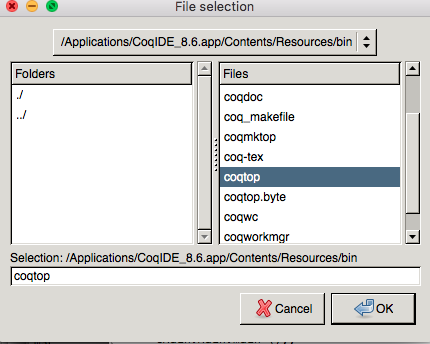
\includegraphics[scale=0.5]{Installation/macos.png}
\caption{Choose the Coq app in a Mac env}\label{fig:macos}
\end{figure}
\item enjoy

\end{enumerate}

\subsection{Windows}
\begin{enumerate}

\item get the zipfile spatchcoq.zip,  unzip it in a folder on a usb stick and doubleclick the application file spatchcoq. 
Note this version includes an instalation of Coq (not very extensively tested yet)

\item enjoy
\end{enumerate}


\subsection{Linux}
\begin{enumerate}
\item Download and install  the latest version of Coq it needs to be at least 8.6 so do not use 
apt-get install coq
\item  go to https://github.com/corneliuhoffman/spatchcoqocaml/tree/master
to build from scratch.
\item when prompted go to the Coq folder you just installed with opam and find  the application called {\bf coqtop}

\item enjoy
\end{enumerate}










